\begin{frame}{SGIRI: dónde usamos servicios web}
\begin{columns}[c]
\begin{column}{0.42\textwidth}
\small
\begin{itemize}
\item Registra los tickets de soporte de una empresa: el cliente cuenta la falla, el administrador asigna un técnico y el técnico cierra con evidencias.
\item El front está en Angular, el servidor en Spring Boot y los datos en PostgreSQL.
\item Se apoya en dos servicios de internet: Globalping mide la red y Cloudinary guarda las fotos.
\end{itemize}
\end{column}
\begin{column}{0.56\textwidth}
\centering
\begin{tikzpicture}[caja/.style={draw=verde,rounded corners=3pt,fill=verdesuave,minimum width=2.2cm,minimum height=0.8cm,font=\scriptsize,align=center}, flecha/.style={-{Stealth[length=2.2mm]},thick,color=tinta}, etiqueta/.style={font=\tiny,color=gris}]
\node[caja] (front) at (0,1.7) {Angular\\(cliente)};
\node[caja] (back) at (0,0.5) {Spring Boot\\(servidor)};
\node[caja] (bd) at (-2.7,-0.9) {PostgreSQL};
\node[caja] (gp) at (0,-0.9) {Globalping};
\node[caja] (cl) at (2.7,-0.9) {Cloudinary};
\draw[flecha] (front) -- node[right,etiqueta]{JSON} (back);
\draw[flecha] (back) -- (bd);
\draw[flecha] (back) -- node[right,etiqueta]{internet} (gp);
\draw[flecha] (back) -- (cl);
\end{tikzpicture}
\end{column}
\end{columns}
\end{frame}

\begin{frame}{Una petición real a la API de SGIRI}
\centering
\IfFileExists{../figuras/mendoza-peticion.png}{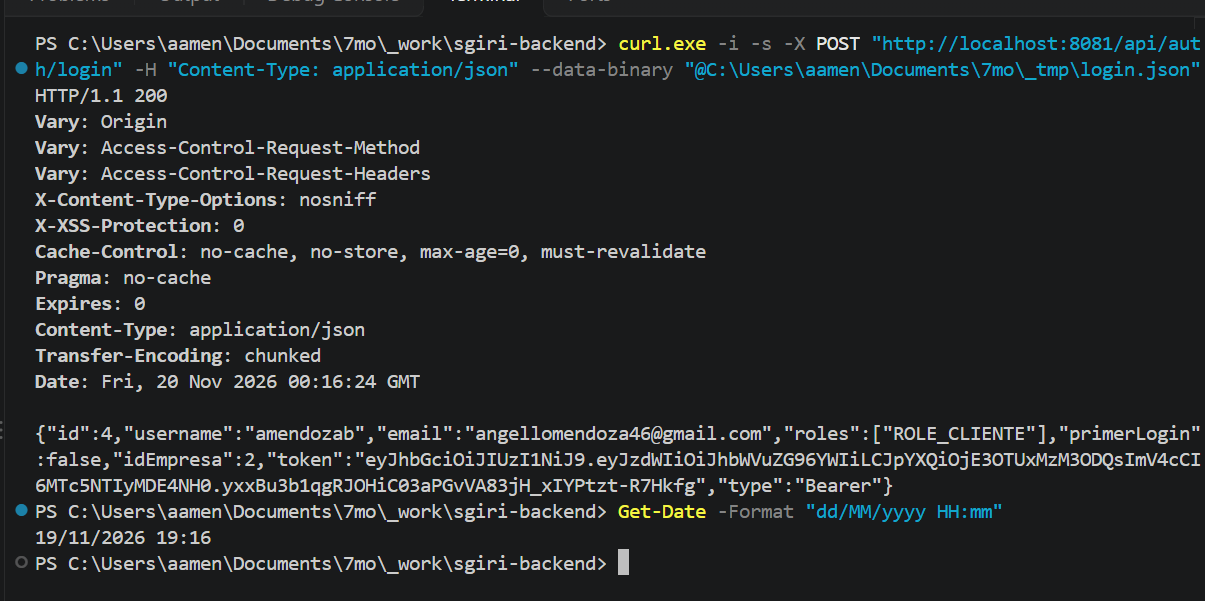
\includegraphics[width=0.78\linewidth,height=0.58\textheight,keepaspectratio]{../figuras/mendoza-peticion.png}}{\fbox{\parbox[c][4.4cm][c]{0.95\linewidth}{\centering\small\color{gris}Falta \texttt{figuras/mendoza-peticion.png}: captura de la petición con la fecha visible}}}
\par\vspace{4pt}
{\scriptsize \texttt{POST /api/auth/login} devuelve 200 con el usuario, su rol y el token; con ese token se piden los tickets.}
\fuente{rfc9110}
\end{frame}

\begin{frame}{Cuando el servicio externo falla}
\begin{columns}[c]
\begin{column}{0.6\textwidth}
\centering
\begin{tikzpicture}[paso/.style={draw=verde,rounded corners=3pt,fill=verdesuave,minimum width=2.5cm,minimum height=0.9cm,font=\scriptsize,align=center}, flecha/.style={-{Stealth[length=2.2mm]},thick,color=tinta}, falla/.style={font=\tiny,color=rojo}]
\node[paso] (a) {IPv4\\Ecuador};
\node[paso,right=0.35cm of a] (b) {IPv6\\Ecuador};
\node[paso,right=0.35cm of b] (c) {IPv4\\Sudamérica};
\node[paso,below=0.75cm of b,minimum width=4.4cm] (d) {intento fallido + último dato bueno};
\draw[flecha] (a) -- node[above,falla]{falla} (b);
\draw[flecha] (b) -- node[above,falla]{falla} (c);
\draw[flecha] (c) |- (d);
\end{tikzpicture}
\end{column}
\begin{column}{0.36\textwidth}
\footnotesize
\begin{itemize}
\item Pide la medición y la consulta cada 2 segundos.
\item Si nada responde, guarda el intento como fallido.
\item El mapa sigue mostrando el último dato bueno.
\end{itemize}
\end{column}
\end{columns}
\vspace{4pt}
\begin{block}{Lo que aprendimos}
SGIRI no esconde el fallo: lo deja anotado y sigue mostrando el último dato. El riesgo es que ese dato ya esté viejo, aunque la pantalla muestre la fecha.
\end{block}
\fuente{rfc9110}
\end{frame}
